\lecture{6}{12. Februar 2025}{Mechanical Properties, Pt. 1: Elasticity}
From physics we are already familiar with the concept of springs. These are defined in terms of a so-called Spring constant that measures the ``stiffness'' of a spring. For general notes on spring systems please see the lecture-notes for ``Physics and Mechanics'' from the 1st semester.

\section{Elasticity}

\subsection{Force-displacement relation}
A Force-displacement relation is the relation between the applied force and the resulting displacement for a given material. This is, however, a rather ungeneralized notion as it does not take into account the thickness or general dimensionality of the test-specimen meaning the result is only true for a given material with a given shape/size. Instead we will seek to define stress and strain as an internal and relative measure of the force and displacement, respectively.

\subsection{Strain}
Strain $\epsilon$ is a relative measurement of displacement. It is given by
\[ 
\epsilon = \frac{d}{L_0}
.\]
Where $d$ is the measured displacement and the gauge length, $L_0$ is the \textit{original} length of the material -- it should be noted that for the common ``wishbone''-geometry of Tensile test-specimens $L_0$ is typically taken to be a length slightly shorter than the length of the narrow section in the middle as the thick ends will not expand as much (the error goes to zero as the geometry goes to infinitely crazy). Strain is a unit-less scalar, although the unit of strain is sometimes given as $[\epsilon] = \unit{\frac{mm}{m}}$ to compensate for (often) very small numbers.

\subsection{Stress}
Stress $\sigma$ is a relative measurement of force. It is given by
\[ 
\sigma = \frac{F}{A_0}
.\]
Where $F$ is the applied force and $A_0$ is the cross sectional area of the specimen. Stress has units of \unit{Pa} or \unit{N/m^2} and it is therefore commensurable to pressure. Stresses are often in an order of about $\qty{1e6}{Pa}$ and therefore $[\sigma]$ is often given as \unit{MPa}.

\subsection{Stress-strain relations}
We will now seek to find a relation between the two quantities of stress and strain. We start by imagining a rod subject to a force. It is a reasonable expectation that the rod will act sort of in the same way as a spring. We will therefore use the formula for the force in a spring as
\[ 
F = kd
.\]
We can now rewrite this as
\[ 
\frac{F}{A_0} A_0 = k \frac{d}{l_0} l_0
.\]
And it becomes obvious the above is just
\[ 
\sigma A_0 = k \epsilon l_0
.\]
This can be written as
\[ 
\sigma = \frac{k l_0}{A_0} \epsilon
.\]
By introducing the Modulus of Elasticity (Young's modulus) $E = \frac{k l_0}{A_0}$ we can write the above as
\[ 
\sigma = E \epsilon \implies E = \frac{\sigma}{\epsilon}
.\]
Now we have found a constitutive equation between stress $\sigma$ and strain $\epsilon$ only depending on the (\textit{material-specific}) elastic modulus $E$.

\subsection{Elatic deformation}
\textit{Elastic deformation} is non-permanent and reversible. It is generally the type of deformation happening at small deformations and the stress/strain curve is approximately linear (with the elastic modulus $E$ as its slope). On a microscopical scale elastic deformation can be thought about as a ``stretching'' of the interatomic bonds -- this ``stretching'' will stop when the applied force is removed.

\subsubsection{Elastic modulus and interatomic bonding forces}
The elastic modulus $E$ depends on the strength of the interatomic forces in the material. Actually, the modulus of elasticity is proportional to the slope of the interatomic force-interatomic seperation curve as shown in \textbf{\autoref{fig:f6_1}} -- also it is true that in general we get that $E \propto r_0^{-2}$, where $r_0$ is the equilibrium interatomic spacing. Elastic moduli for different common materials are shown in \textbf{\autoref{fig:f6_2}}.
\begin{figure} [ht]
  \centering
  \caption{Relationship between EM and interatomic interactions}
  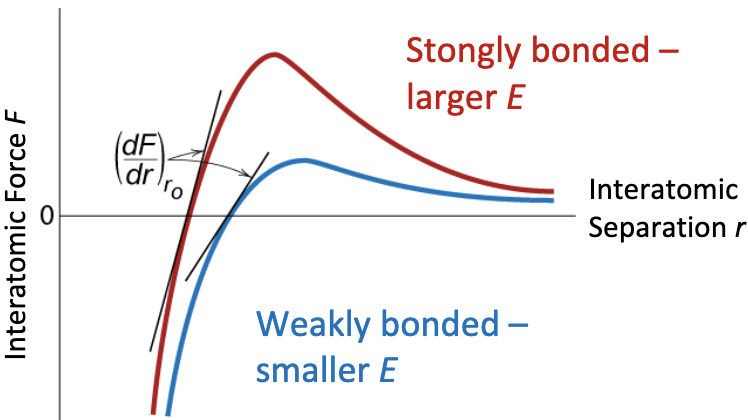
\includegraphics[width=0.5\linewidth]{./figures/f6_1.png}
  \label{fig:f6_1}
\end{figure}
\begin{figure} [ht]
  \centering
  \caption{EM for common materials ($y$-axis is given in MPa)}
  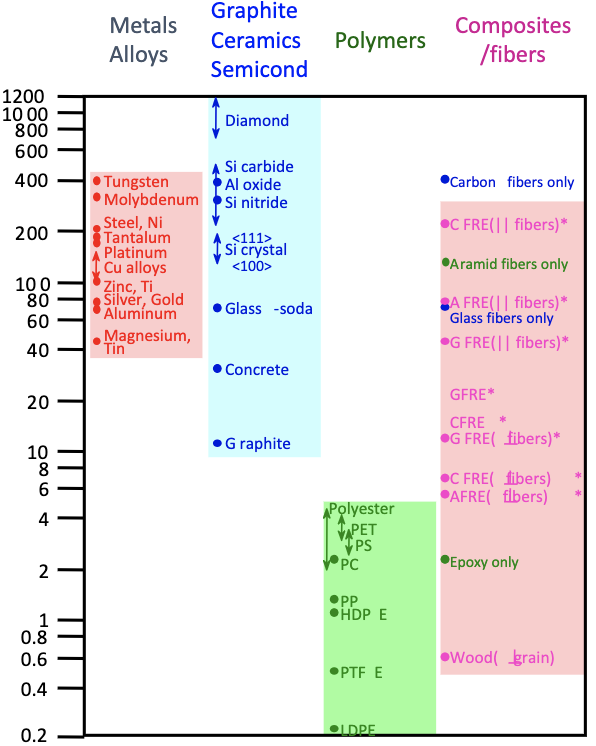
\includegraphics[width=0.35\linewidth]{./figures/f6_2.png}
  \label{fig:f6_2}
\end{figure}

\subsection{Shear stress}
Not always the \textit{tensile} version of stress is wanted. Sometimes one instead seeks to find a solution to a problem involving a ``bending'' of the material. This is known as shear stress $\tau$. Shear stress is also given as
\[ 
\tau = \frac{F_{\perp}}{A_0}
.\]
As was the case for tensile stress we also want to find a constitutive equation for shear stress. We once again start as
\[ 
F = k d
.\]
And follow the same steps as was the case for the tensile stress until we get
\[ 
\tau = \frac{k l_0}{A_0} \gamma
.\]
Where $\gamma = \frac{d}{l_0}$ is the shear strain and $\tau$ is the shear stress. We now define $G = \frac{k l_0}{A_0}$ as the shear modulus and get
\[ 
\tau = G \gamma
.\]
The tensile modulus $E$ is always larger than the shear modulus $G$.
\[ 
E > G
.\]

\subsubsection{Stresses on different planes}
To compute a stress, a specific plane needs to be defined. This is shown in \textbf{\autoref{fig:f6_3}}.
\begin{figure} [ht]
  \centering
  \caption{Stresses on different planes}
  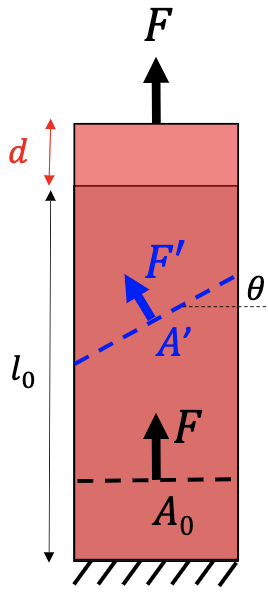
\includegraphics[width=0.15\linewidth]{./figures/f6_3.png}
  \label{fig:f6_3}
\end{figure}
For the case on \textbf{\autoref{fig:f6_3}} we actually get the two relations for the tensile stress
\begin{align*}
  \sigma_0 &= \frac{F}{A_0} \\
  \sigma' &= \frac{F'}{A'}
.\end{align*}
These two tensile stresses are related by
\[ 
\sigma' = \frac{F \cos\theta}{A_0 / \cos\theta} = \sigma_0 \cos^2\theta = \sigma_0 \left( \frac{1 + \cos 2\theta}{2} \right)
.\]
And the shear stresses are related as
\[ 
\tau' = \frac{F \sin\theta}{A_0 / \cos\theta} = \sigma_0 \sin\theta \cos\theta = \sigma_0 \left( \frac{\sin 2\theta}{2} \right)
.\]

\subsection{Bulk modulus}
The \textit{bulk modulus} $K$ is a measurement of how resistant a material is to compression and it is defined as the ratio of the pressure increase to the resulting relative decrease of the volume.
\[ 
\Delta p = K \frac{\Delta V}{V_0}
.\]

\subsection{Poisson's ratio}
To define the so-called Poisson's ratio we will first define the axial strain $\epsilon_z$ and the transverse strain $\epsilon_x$ as
\begin{align*}
  \epsilon_z &= \frac{d_z}{l_{0_z}} \\
  \epsilon_x &= \frac{d_x}{l_{0_x}}
.\end{align*}
That is the strain in a given direction is defined as the strain measured solely in that direction.

Poisson's ratio $\nu$ is then defined as
\[ 
\nu = - \frac{\epsilon_x}{\epsilon_z}
.\]
The Poisson's ratio is thus a measurement of the Poisson effect, which is the deformation (expansion or contraction) of a material in the directions perpendicular to the applied load.

\subsubsection{The relationship between Poisson's ratio and moduli}
It can be shown that
\[ 
G = \frac{E}{2(1+\nu)} \quad \text{and} \quad K = \frac{E}{3(1-2\nu)}
.\]
That means the shear and bulk moduli ($G$ and $K$) can be found in terms of the Poisson ratio $\nu$ and Youngs modulus $E$. This also means that the Poisson's ratio of a stable, isotropic, linear elastic material must be between $-1$ and $+0.5$, because of the requirement for Young's, shear and bulk modulus to have positive values. A negative Poisson's ratio indicate that the material expands when a perpendicular force is applied and therefore most materials have positive Poisson's ratio -- All materials with negative Poisson's ratios are known under the name \textit{Auxetics}.
